\subsubsection{\theoryC{High mass $t\bar{t}$ resonance search at HE-LHC}}
\label{subsec:topreso:HELHC}
\contributors{C. Helsens, D. Jamin, M. Selvaggi}\rt{There are comments to address.}
%{\bf Authors: C. Helsens$^1$, D. Jamin$^2$, M. Selvaggi$^3$}\\
%\newline
%$^1$CERN EP-Departement, CH-1211 Geneva 23, Switzerland email: {\tt B.C. clement.helsens@cern.ch}\\
%$^2$Academia Sinica, Institute of  Physics, Taipei, Taiwan\\

%\newcommand*{\zptt}{\ensuremath{Z^{\prime} \rightarrow \ttbar}}
%\newcommand*{\qjj}{\ensuremath{Q^{*} \rightarrow jj}}
%\newcommand*{\rsg}{\ensuremath{G_{RS} \rightarrow WW}}
%\newcommand*{\vj}{\ensuremath{\text{V + jets}}}
%\newcommand*{\ZpSSM}{\ensuremath{Z^{\prime}_{\mathrm{SSM}}}}
%\newcommand*{\metvec}{\vec{\pt}^{\textrm{miss}}}
%\newcommand*{\intlumihelhc}{\ensuremath{\mathcal{L}=15\text{ ab}^{-1}}}

%\textbf{Reponsible: Clement Helsens, Michele Selvaggi}

%%%%%%%%%%%%%%%%%%%%%%%%%%%%%%%%%%%%%%%%%%%%%%%%%%%%%%%%%%%%%%%%%%%%%%%%%%%%%%%%%%%%%%%%%%%%
%\subsubsection{Introduction}
%\paragraph*{Introduction}
Several BSM models predict additional particles with masses at the TeV scale. The presence of new resonant states~\cite{Harris:2011bh,Boelaert:2009jm,Lee:1973iz,Branco:2011iw,Hill:1994hp,Kaplan:1983sm,Bellazzini:2014yua,Randall:1999ee,Pomarol:1999ad} decaying to a pair of top quarks could be observed as an excess over the SM background in the ditop invariant mass distribution. We focus here on the specific benchmark model of a Sequential Standard Model \ZpSSM~\cite{Langacker:2008yv}. \rt{From the figure it seems that also a $Z'_{\text{TC2}}$ is used.} We study the sensitivity in the following decay using the hadronic \zptt\ decay mode. \rt{At the end of the contribution there is a table that is never mentioned nor commented. Needs to be completed.}

The decay products are typically in the multi-TeV regime and their reconstruction imposes stringent requirement on the detector design. Precise jet energy resolution requires full longitudinal shower containment. Highly boosted top quarks decay into highly collimated jets that need to  be disentangled from standard QCD jets by studying their substructure. High discrimination power and sensitivity for this search at such extreme energies, requires excellent granularity both in the tracking detectors and calorimeters.

%%%%%%%%%%%%%%%%%%%%%%%%%%%%%%%%%%%%%%%%%%%%%%%%%%%%%%%%%%%%%%%%%%%%%%%%%%%%%%%%%%%%%%%%%%%%
%\subsubsection{Monte Carlo Samples}
%\paragraph*{Monte Carlo Samples}
Signal models were generated at the LO with \PYTHIA~8.230~\cite{Sjostrand:2014zea}. The SM backgrounds are dijet (QCD), top pairs ($\ttbar$), $VV$ and $V+\text{jets}$ where $V=W/Z$, and have been generated at LO using \MGvATNLO ~2.5.2~\cite{Alwall:2014hca}. A k-factor of 2 is applied to all the background processes. \rt{This does not make much sense.}


%%%%%%%%%%%%%%%%%%%%%%%%%%%%%%%%%%%%%%%%%%%%%%%%%%%%%%%%%%%%%%%%%%%%%%%%%%%%%%%%%%%%%%%%%%%%
%\subsubsection{Multivariate tagger}
%\paragraph*{Multivariate tagger}
\label{sec:mvatagger}
An important ingredient of the \zptt\ search is the identification of heavy boosted top quarks. A jet tagger using Boosted Decision Trees (BDTs) was developed to discriminate top jets against the dijet background.
%NB: Need to define if more material needed.

%Top and $W$ taggers were optimised using jets with a transverse boost of $\pt=$10 TeV. At these extreme energies, $W$ and top jets have a characteristic angular size $R=0.01-0.02$, i.e smaller than the typical electromagnetic and hadronic calorimeter cells. Following the approach described in \citeref{Larkoski:2015yqa}, we exploit the superior track angular resolution and reconstruct jets from tracks only (track jets) using the anti-$k_T$ algorithm with a parameter R=0.2. The missing neutral energy is corrected for by rescaling the track 4-momenta by the factor $\ptSup{trk}/\ptSup{PF}$, where $\ptSup{trk}$ is the track Jet \pt\ and $\ptSup{PF}$ is the Particle-Flow Jet \pT. In what follows, we will simply refer to ``track jets'' as the jet collection that includes the aforementioned rescaling.
%
%The boosted top tagger is built from jet substructure observables: the soft-dropped jet mass~\cite{Larkoski:2014wba} and N-subjettiness~\cite{Thaler:2010tr} variables $\tau_{1,2,3}$ and their ratios $\tau_{2}/\tau_{1}$ and $\tau_{3}/\tau_{2}$. The $W$-jet versus QCD-jet tagger also uses an ``isolation-like'' variable that exploits the absence of high \pt\ final state-radiation (FSR) in the vicinity of the $W$ decay products. We call these variables $E_{F}(n,\alpha)$ and define them as:
%
%\begin{equation}
%E_{F}(n,\alpha) =  \frac{\sum \limits_{\frac{n-1}{5}\alpha < \Delta R(k,jet)< \frac{n}{5}\alpha} \ptSup{(k)}}{\sum \limits_{\Delta R(k,jet)< \alpha} \ptSup{(k)}}
%\end{equation}
%
%We use $\alpha=0.05$. We construct 5 variables $E_{F}(n,\alpha)$ with $n=1..5$ and provide them as input to the BDT. The $E_{F}(1,0.05)$ observable is shown in \fig{fig:hadronicresonances:BDTeff} (left).
%The final performance of the $W$ and top tagger is shown in \fig{fig:hadronicresonances:BDTeff} (right). The $W$ tagging performance has significantly better performance due to the use of the energy-flow variables. We choose our working points with a top and $W$ tagging efficiencies of $\epsilon_S^{\text{top}}=60\%$ and $\epsilon_S^{\text{W}}=90\%$ corresponding respectively to a background efficiency of $\epsilon_B^{\text{top}}=\epsilon_B^{\text{W}}=10\%$.
%
%
%\begin{Figure}
%  \centering
%  \includegraphics[width=0.37\columnwidth]{\main/img/hadronicresonances/Jet1_Flow15_sel0_nostack_logx.eps}
%  \includegraphics[width=0.45\columnwidth]{\main/img/hadronicresonances/effQCD_vs_effWhadBlue_thadRed_log.eps}
%  \caption{Left: Energy-flow ($E_{F}(1,0.05)$) observable for W and QCD jets. Right: Dijet rejection versus signal efficiency for the two taggers, W in blue and top in red.%\MS{need editing - REDO left EFlow in logX - Right: need legend and stars}
%  }
%  \label{fig:hadronicresonances:BDTeff}
%\end{Figure}

%%%%%%%%%%%%%%%%%%%%%%%%%%%%%%%%%%%%%%%%%%%%%%%%%%%%%%%%%%%%%%%%%%%%%%%%%%%%%%%%%%%%%%%%%%%%
%\subsubsection{Event Selection}
%\paragraph*{Event Selection}

The jet selection for the \zptt\ search is using track jets, as these are better at resolving the jet sub-structure compared to particle-flow jets. Since no lepton veto is applied, there is also some acceptance for leptonic decays. The sensitivity to semi-leptonic $\ttbar$ decays is enhanced by adding the $\metvec$ vector to the closest jet 4-momentum (among the two leading jets).

We require two jets with $\pt>1$~TeV, $|\eta<3|$ and $\Delta\eta<2.4$. Both jets must be top tagged. Both high-$\pt$ jets must be $b$-tagged.\rt{Here is unclear. Which jets should be top and b-tagged?} Finally, to further reject the QCD background, we require for both jets $m_{SD}>40$~GeV. \rt{What is $m_{SD}$?} In left panel of \fig{fig:hadronicresonances:ttsel08} we show the dijet invariant mass distribution after the final analysis cuts. \rt{Right fig $\sqrt{s}$ not properly shown. Middle and right figs labels should be HE-LHC and not HELHC. Also the label is outside for the left fig and inside for the other two. Can this be made uniform?}
\begin{figure}[tbp]
  \centering
  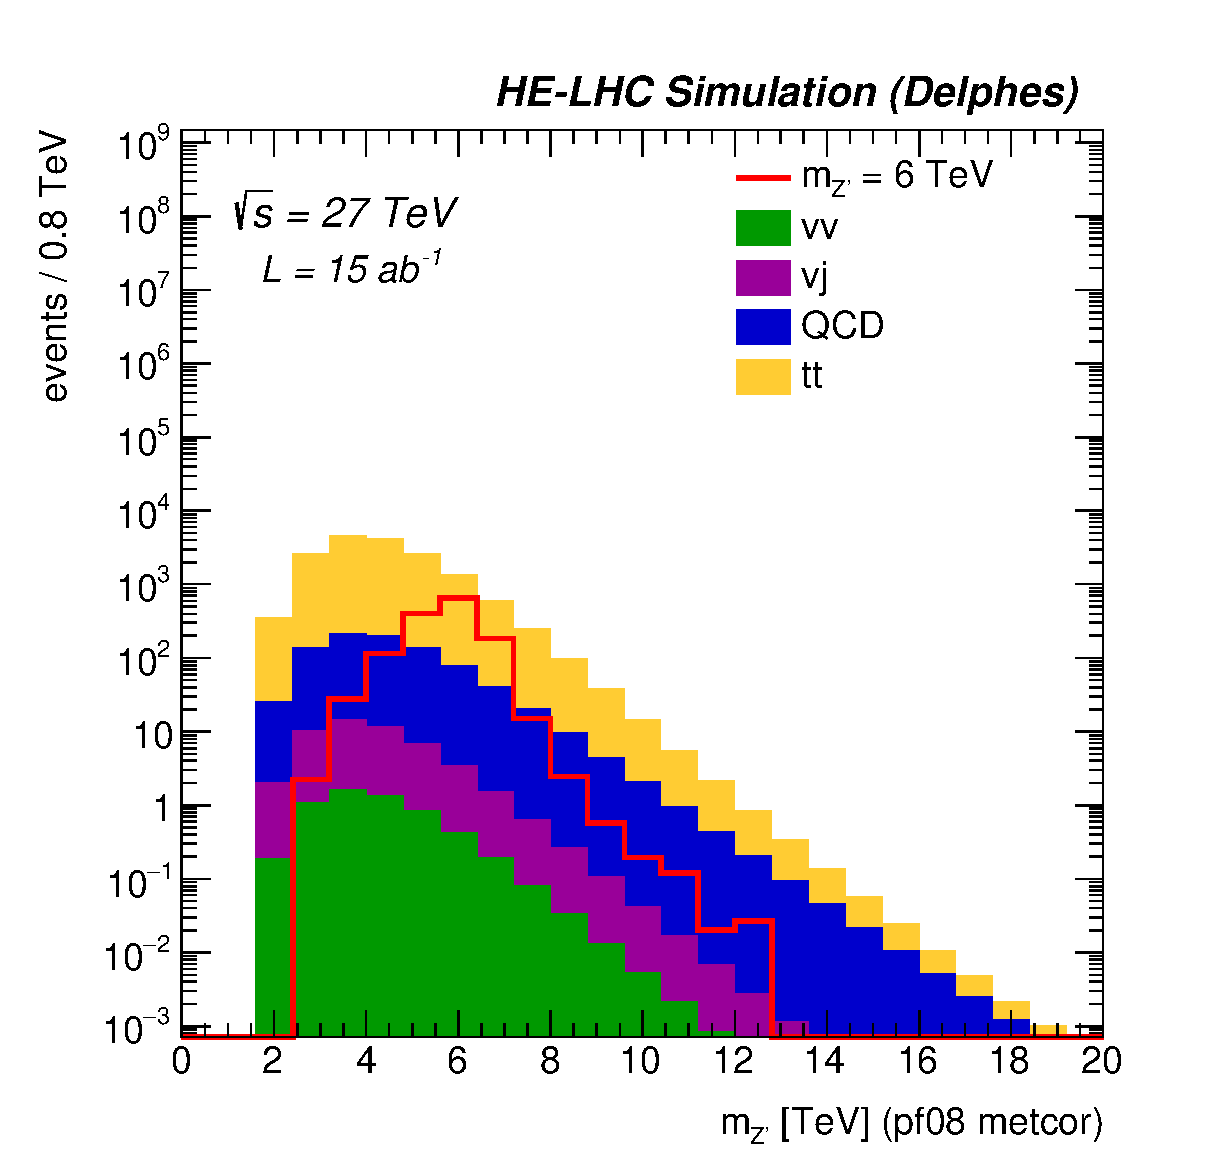
\includegraphics[width=0.32\columnwidth]{\main/section7OtherSignatures/img/Zptt_Mj1j2_pf08_MetCorr_fit_sel8_nostack_log.eps}
  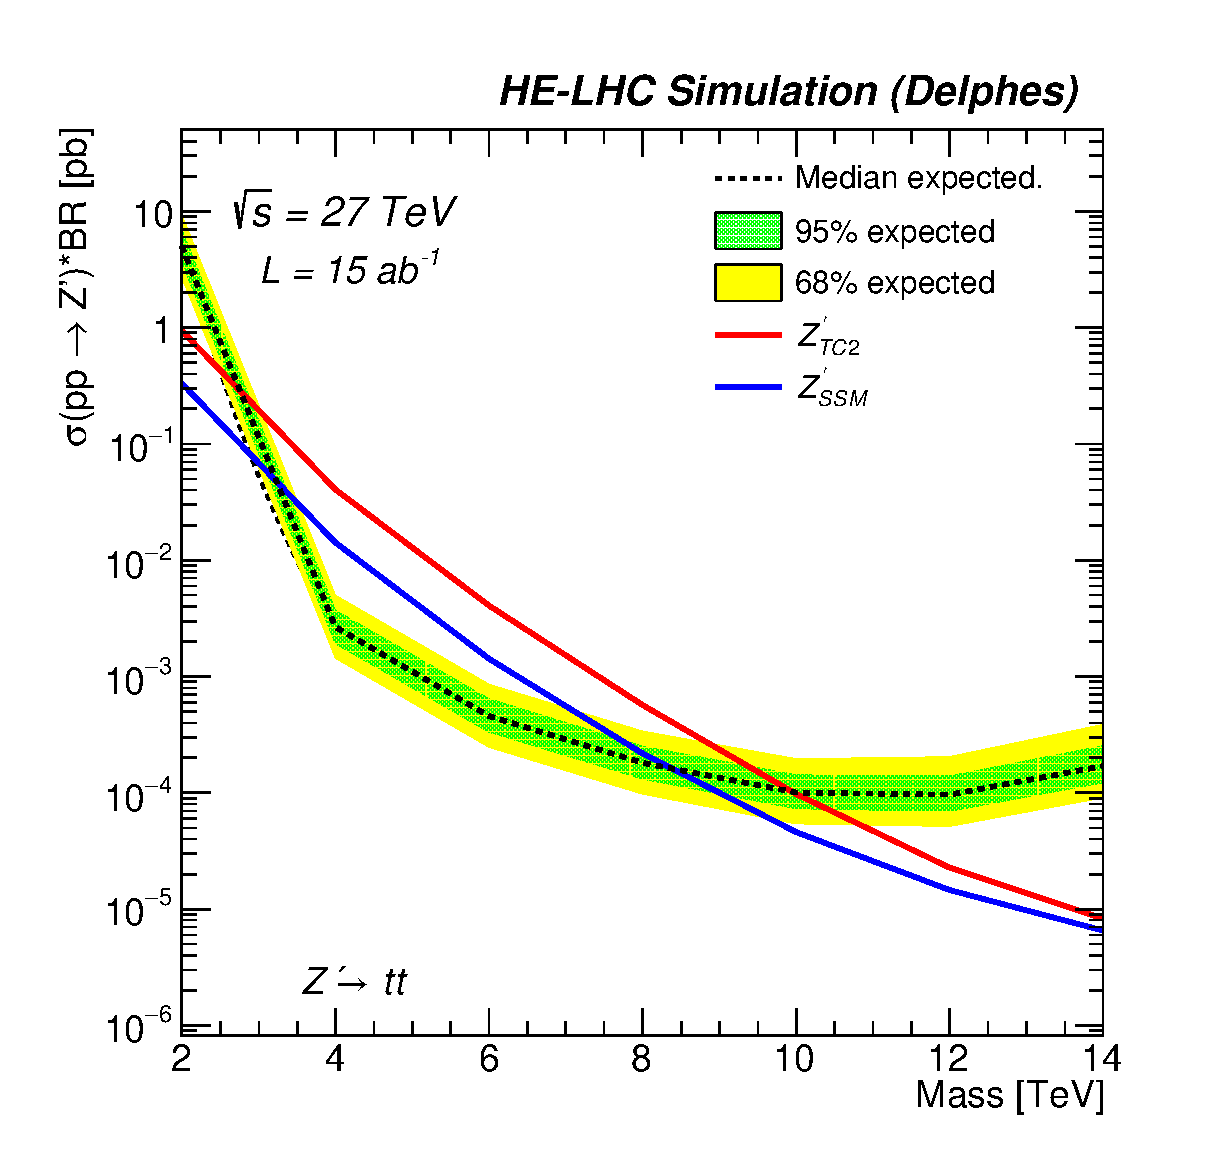
\includegraphics[width=0.32\columnwidth]{\main/section7OtherSignatures/img/lim_Zprime_tt_helhc_v01.eps}
  \includegraphics[width=0.32\columnwidth]{\main/section7OtherSignatures/img/DiscoveryPotential_tt_SSM_TC2_tagger_TRFbtag_rootStyle.eps}
  \caption{Left distribution : invariant mass distribution of the two leading jets for the full selection for a 6~TeV signal for the \zptt\ analysis. Middle distribution : exclusion limit at 95\%~\cl versus heavy resonance mass. Right distribution : integrated luminosity for a $5\sigma$ discovery as a function of the heavy resonance mass.}
  \label{fig:hadronicresonances:ttsel08}
\end{figure}

%%%%%%%%%%%%%%%%%%%%%%%%%%%%%%%%%%%%%%%%%%%%%%%%%%%%%%%%%%%%%%%%%%%%%%%%%%%%%%%%%%%%%%%%%%%%
%\subsubsection{Signal extraction and results}
%\paragraph*{Signal extraction and results}
Hypothesis testing is performed using a modified frequentist method based on a profile likelihood fit that takes into account the systematic uncertainties as nuisance parameters. The dijet invariant mass is used as a discriminant. In order to reduce large statistical fluctuations from high Monte Carlo weight events, we parameterize the background invariant mass distribution with the following function (conservatively assuming 50\% uncertainty on the background normalisation) $f(z)=p_1(1-z)^{p_2}z^{p_3}z^{p_{4}logz}$, where $z=m_{jj}/\sqrt{s}$, and the $p_{i}$ are free parameters.

The expected exclusion limit at 95\%~\cl and discovery reach at $5 \sigma$ are shown in the middle and right panels of \fig{fig:hadronicresonances:ttsel08}. Reconstructing heavy resonances decaying to $\ttbar$ is challenging and requires the use of novel approaches to boosted object tagging to reduce the backgrounds. The reach for \zptt\ (in TC2 models) is 10~TeV with \intlumihelhc and it is possible to discover it up to $m_{Z}=8$~TeV. \rt{Before only SSM $Z'$ was mentioned. Now only TC2 $Z'$ reach is quoted. Needs to be completed.} 

\begin{table}[!htb]\centering
\scalebox{0.9}{
\begin{tabular}{|c|c|c|}
\hline
\hline
signal $m_{Z}$  & 2 TeV  &    84.0 \\
                & 4 TeV  &  4702.8 \\
                & 6 TeV  &  1401.9 \\
                & 8 TeV  &   215.5 \\
                & 10 TeV &    27.6 \\
                & 12 TeV &     3.8 \\
                & 14 TeV &     0.8 \\
\hline
background      & vv     &     5.9 \\
                & vj     &    45.7 \\
                & tt     &   827.4 \\
                & QCD    & 15909.0 \\
                & total  & 16788.0 \\
\hline
\hline
\end{tabular}}
\caption{Final yield of analysis.}
\label{tab:ZpttYield}
\end{table}
